\documentclass[main.tex]{subfiles}
\begin{document}

\begin{comment}

\section{Study}

\begin{itemize}
\item cloud versus edge
\item gradient descent
\itme perceptron
\item hashing
\item signal processing
\item matrix computation
\item operation benchmarks, operation per system per joule
\item generative adversarial neural networks
\end{itemize}

\subsection{Introduction}
\subsection{Supervised ML}
Probabilistic Learning Model
$$\epsilon \triangleq \mathbb{E}_{(x, y) \sim \mathcal{D}}[\ell(y, f(x))]=\sum_{(x, y)} \mathcal{D}(x, y) \ell(y, f(x))$$
Our training error is simply our average error over the training data. 
$$\hat{\epsilon} \triangleq \frac{1}{N} \sum_{n=1}^{N} \ell\left(y_{n}, f\left(\boldsymbol{x}_{n}\right)\right)$$

\subsection{Perceptron}
Input vector $X_i$, weights $w_i$, bias $b$, activation function $f$
$$f\left(\sum_{i} w_{i} x_{i}+b\right)$$

\begin{algorithm}
\caption{PerceptronTrain(\textbf{D}, MaxIter)}
\begin{algorithmic}[1]
\State $w_d \leftarrow 0, \text{ for all } d = 1 ... D$ 
\State $b \leftarrow 0$
\For{$iter = 1 ... MaxIter$}
    \ForAll{$(x, y) \in \mathbf{D}$}
        \State $a \leftarrow \sum_{d=1}^{D} w_d x_d +b$
        \If{$ya \leq 0$}{
            \State $w_d \leftarrow w_d + yx_d, \text{ for all } d = 1...D$
            \State $b \leftarrow b + y$
        \EndIf
    \EndFor
\EndFor
\State \Return $w_0, w_1, ..., w_D, b$
\end{algorithmic}
\end{algorithm}

Decision boundary where activation changes from -1 to +1
$$\mathcal{B}=\left\{x: \sum_{d} w_{d} x_{d}=0\right\}$$

\subsubsection{Spiking Neural Networks}
Signals are idieally represented by series of delta functions where the inputs and outputs, for spike times $\tau_j$ take the form 
$$x(t)=\sum_{j=1}^{n} \delta\left(t-\tau_{j}\right)$$

\subsection{Neural Networks}
\subsubsection{Gradient Decent}
Define differentiable function $F(x)$ with gradient $\nabla F\left(\mathbf{x}_{n}\right)$ and step on gradient $-\gamma_{n} \nabla F\left(\mathbf{x}_{n}\right)$ where

$$\gamma_{n}=\frac{\left|\left(\mathbf{x}_{n}-\mathbf{x}_{n-1}\right)^{T}\left[\nabla F\left(\mathbf{x}_{n}\right)-\nabla F\left(\mathbf{x}_{n-1}\right)\right]\right|}{\left\|\nabla F\left(\mathbf{x}_{n}\right)-\nabla F\left(\mathbf{x}_{n-1}\right)\right\|^{2}}$$

and where $\gamma \in \mathbb{R}_{+}$ and $n \in N>0$ which equals the number of steps. With an initial guess $x_0$, and a sequence of steps $\mathbf{x}_{0}, \mathbf{x}_{1}, \mathbf{x}_{2}, \ldots$, such that 

$$\mathbf{x}_{n+1}=\mathbf{x}_{n}-\gamma_{n} \nabla F\left(\mathbf{x}_{n}\right), n \geq 0$$

resulting in a monotonic sequence $F\left(\mathbf{x}_{0}\right) \geq F\left(\mathbf{x}_{1}\right) \geq F\left(\mathbf{x}_{2}\right) \geq \cdots$ that converges to a desired local minimum.

\subsubsection{Back Propagation}

\begin{aligned}
&\delta^{L}=\nabla_{a} C \odot \sigma^{\prime}\left(z^{L}\right) \\
&\delta^{l}=\left(\left(w^{l+1}\right)^{T} \delta^{l+1}\right) \odot \sigma^{\prime}\left(z^{l}\right) \\
&\frac{\partial C}{\partial b_{j}^{l}}=\delta_{j}^{l} \\
&\frac{\partial C}{\partial w_{j k}^{l}}=a_{k}^{l-1} \delta_{j}^{l}
\end{aligned}

\subsubsection{Nonlinear Activation Function (NLAF)}

Logistic function where $x_0$, the $x$ value of the sigmoid's midpoint, $L$, the curve's maximum value, $k$, the logistic growth rate or steepness of the curve resulting in 

$$f(x)=\frac{L}{1+e^{-k\left(x-x_{0}\right)}}$$

\subsection{Introduction Theory}

\subsubsection{Communication Limits}
Shannon limit $C \sim \log _{2}(1+S N R)$, Density in electrical interconnects $B \propto A / \ell^{2}$

\subsubsection{Communication Limits}
Options for multiplexing, signal noise ratio (SNR) $\mathrm{C} \sim \mathrm{M} \times \mathrm{B} \times 2 \log _{2}(\mathrm{SNR})$

\subsection{Hardware for AI}
Biological Plausibility $x(t)=\sum_{j=1}^{n} \delta\left(t-\tau_{j}\right)$
\subsection{Optics for AI}
Montgomery Multiplication $\bar{C}=\frac{\bar{a} \bar{b}+\left(\bar{a} \bar{b} M^{-1} \bmod R\right) M}{R}$

\subsection{Photonic Integrated Hardware}

\end{comment}

\section{Joseph Crandall Midterm}

\subsection{Warm-ups}
\begin{enumerate}

\item A key feature of neural network for AI is that they offer train ability. Briefly (1-2 sentences) state \textbf{Q a)} why is training essential for "learning" such as in machine learning. \textbf{A a} Training is the learning process by which the weights in your perceptron (core building block of NN) get rewritten based on activation function. This process is iterative and allows the algorithm to improve on its classification of data points. Training more generally in learning is iteratively trying a solution, testing it against a known truth, and then modifying your value to improve your results. \textbf{Q b)} Then, discuss (2-3 sentences) what challenges exist when training neural networks. \textbf{A b} one of the core challenges in training is over fitting, this is the process where you create an decision boundary in your data set that two closely represents that data set that you have been training on. The result is that the trained model does not generalize well because when you pass it novel data it categorizes it based almost entirely on the unique data you used during training. Another challenge in training is the type of non-linear activation function that you use to decide if a value is correct or incorrect and therefore requires additional iterative modification. The wide variety of mathematical functions available means that you must develop a deep understand of the modality of data you are using and the characteristics of it that make that NLAF useful.

\item For training a perceptron or neural network, the neurons(s) perform a weighted sum of the input vectors. \textbf{Question:} if $y = \vec{y}\vec{x}$ correct, or $y=\vec{w^T}\vec{x}$? Tip: here the bold annotation refers to a vector and the superscript T to the transposed vector (also known as 'augmented'). State your answer either by explaining, or a calculation. \textbf{A} For the peceptron the Input vector $X_i$, weights vector $w_i$, bias $b$, activation function $f$ are defined as follows
$$f\left(\sum_{i} w_{i} x_{i}+b\right)$$

If both vectors for example are 4x1, then you would need the technically you would need the transpose of the weights vector so you could perform a 1x4 X 4x1 matrix (vector) multiplication.

\item Neural networks are not new, and are in fact known since the 1950's. Why do we have an AI revolution now? State 3 key factors that are \textbf{a)} required for machine-learning, and \textbf{b} give an actual example (product/name/option etc). \textbf{A} 1. Plentiful data and a desire to monetize that data through prediction products to the same level of success the Google and Facebook were able to in the 2000's through their adds driven business models. 2. The success of Alex Net and other Deep Neural Networks that have been experiencing and parameters explosion since 2012 and have out performed other algorithms at image classification and speed recognition. 3. A large open source community build around python that has made many Machine Learning Neural network algorithms accessable to novice users. 

\item \textbf{Q} Training Algorithm and Non linearity: In class, we discussed training algorithm based on gradient descent algorithm and signal back-propagation. We encountered a possible issue known as vanishing (or exploding) gradients. Briefly state or explain the issue, and then state and briefly discuss a possible solution to it. \textbf{A} For gradient decent you define differentiable function $F(x)$ with gradient $\nabla F\left(\mathbf{x}_{n}\right)$ and step on gradient $-\gamma_{n} \nabla F\left(\mathbf{x}_{n}\right)$ where

$$\gamma_{n}=\frac{\left|\left(\mathbf{x}_{n}-\mathbf{x}_{n-1}\right)^{T}\left[\nabla F\left(\mathbf{x}_{n}\right)-\nabla F\left(\mathbf{x}_{n-1}\right)\right]\right|}{\left\|\nabla F\left(\mathbf{x}_{n}\right)-\nabla F\left(\mathbf{x}_{n-1}\right)\right\|^{2}}$$

and where $\gamma \in \mathbb{R}_{+}$ and $n \in N>0$ which equals the number of steps. With an initial guess $x_0$, and a sequence of steps $\mathbf{x}_{0}, \mathbf{x}_{1}, \mathbf{x}_{2}, \ldots$, such that 

$$\mathbf{x}_{n+1}=\mathbf{x}_{n}-\gamma_{n} \nabla F\left(\mathbf{x}_{n}\right), n \geq 0$$

resulting in a monotonic sequence $F\left(\mathbf{x}_{0}\right) \geq F\left(\mathbf{x}_{1}\right) \geq F\left(\mathbf{x}_{2}\right) \geq \cdots$ that converges to a desired local minimum. The problem arises when you quickly reach a local minimum and your gradient goes to zero. This is fine of your data is generally "convex" in structure meaning that no matter where you start your descent you are roughly guaranteed to arrive at the true minimum. However most data does not have this property and has many local minimums. One solution is to use Stochastic gradient descent where Select initial random guess, but pick additional starting guesses from sample space and repeat finding min for entire data set. From all of these iterations you select the lowest local minimum, which is likely to be closer to the true minimum.

\end{enumerate}

\subsection{Electronic AI Hardware}
\begin{enumerate}
\item Memory
    \begin{enumerate}
    \item \textbf{Q} What is the role of Memory in machine learning and neural networks? What its role in machine intelligence (in general) and learning? \textbf{A} Its primary role is the volatile storage for the purpose of iteratively reading and writing weights as a machine learning algorithm is being trained. In general for machines or other systems to learn, memory allows experiences from the past to be recalled and then used in the present.
    \item \textbf{Q} What performance trade offs exist for memory types (at the physical hardware level). \textbf{A} Memory types can be considered along an axis which starts with volatility (does not persist without power or for very long) read and write time, and storage time, and goes to non volatile, longer read and write times, and larger storage space. Within traditional electronic hardware typically you have multiple layers of volatile caches, followed by random access memory, followed by a jump from volatile to non volatile, followed by disk, and then potentially tapes.
    \item \textbf{Q} ... and how do these trade offs impact AI systems. For example, is an ever-faster WRITE-speed desired for AI systems of a longer retention time. \textbf{A} If you are only using a trained model to make predictions on a data set then fast read times are good, if you are training, then improvements in both read and write times and good, the benefit is that if you can increase your clock speed you can decrease your retation time, however you also need to speed up your time to access the data which can encounter I/O bottle necks.
    \end{enumerate}

    \item AI Systems performance. Refer to the table below, and fill in the missing data and answer the following questions:
    \begin{enumerate}
    \item \textbf{Q} Which AI system has the highest MAC rate? \text{A} MAC $a+(b \times c)$ is defined by inputs times frequency so in this case inputs = signal multiplexing factor times bit resolution, and frequency is clock speed. So system 2 has the highest MAC rate. 
    \item \textbf{Q} Which one is most energy efficient? \text{A} Energy efficiency is defined in GMAC/J, J = Ws, and system MAC rate is in GMAC/s so Efficiency is defined by System MAC Rate / Power Consumption so system 1 is the most efficient. 
    \item \textbf{Q} Which one would you use for a data-center (cloud) vs. which one for a drone (network edge)? Why? You would want to use the efficient system 3 within and edge application, and the inefficient system 1 in the cloud if you have power concerns.
    \item \textbf{Q} Which one do you think could be an electronic system? Which one could be a photonic-accelerated AI system? Why? The 3rd system is most likely photonic since it has the highest clock speed and lowest system latency. The other two are mostly likely electronic.
    
    *Gbps = Giga bits per second = $10^9$ bits per second\\
    **Assume the signal is an on-off keying (OOK). Meaning 1x bit MAC\\
    ***Performing the inference tasks (not training).\\
    
    \end{enumerate}
    \begin{center}
    \begin{tabular}{||c c c c||} 
     \hline
     AI System & Clock speed* (Gbps) & Signal Multiplexing factor & Bit resolution \\ [0.5ex] 
     \hline\hline
     1 & 5 & 1 & 8 \\ 
     \hline
     2 & 1 & 100 & 4 \\
     \hline
     3 & 40 & 4 & 1 \\ [1ex] 
     \hline
    \end{tabular}
    \end{center}
    
    \begin{center}
    \begin{tabular}{||c c c c||} 
     \hline
     AI System & System MAC Rate ** & Power Consumption n (W) & Efficiency (GMAC/J) \\ [0.5ex] 
     \hline\hline
     1 & 40 GMAC/s & 100 & 0.4 \\ 
     \hline
     2 & 400 GMAC/s & 100 & 4 \\
     \hline
     3 & 160 GMAC/s & 10 & 16 \\ [1ex] 
     \hline
    \end{tabular}
    \end{center}
    
    \begin{center}
    \begin{tabular}{||c c c c||} 
     \hline
     AI System & System Latency & Use case \\ [0.5ex] 
     \hline\
     1 & ms & cloud \\ 
     \hline
     2 & us & cloud\\
     \hline
     3 & ns & edge \\ [1ex] 
     \hline
    \end{tabular}
    \end{center}
    
    \item Neuromorphic AI Systems In class we discussed this figure below (not shown).
    \begin{enumerate}
        \item \textbf{Q} Looking at the region (the white box) for 'Neuromorphic Electronics', why are these electronic ASICs so much more efficient as compared to digital compute systems? \textbf{A} The ASICs tend to have fewer I/O interactions with memory, or even disk, and spend more of there time performing the arithmetic of the algorithm without needing to read and write external to the chip.
        \item \textbf{Q} The right side of the figure shows photonic approaches to AI: Why is optical information processing suggested to be so much 'better' than electronics *(either digital or neuromicrphic)? Give several reasons for photonics being superior, and state why electronics has fundamental limits in regards to signal and MAC processing. Finally, what challenges do optical AI hardware accelerators have? \textbf{A}. Bosonic Photons can be clocked in the Terahertz regime, Fermionic electronics would encounter heat issue as these frequencies, photonics can also be multiplexed when adds a physical layer of parallelization that electronics struggles to replicate, and photonics can operate in the atto joule regime.
    \end{enumerate}
    
\end{enumerate}
\subsection{Matrix-Multiplication Drill and Conv. Neural Network for Image Edge Detection}
\begin{enumerate}
    \item \textbf{Q} Perform this matrix-matrix  multiplication. What type of data may the input matrix represent? \textbf{A} Pixel values on a gray scale image.
    
    \begin{bmatrix} 
	1 & 2 & 2 \\
	3 & 4 & 5\\
	6 & 7 & 8 \\
	\end{bmatrix}
	\times
	\begin{bmatrix} 
	4 & 3 & 7 \\
	5 & 5 & 6\\
	3 & 4 & 4 \\
	\end{bmatrix}
	=
	\begin{bmatrix} 
	20 & 21 & 27 \\
	47 & 49 & 65\\
	83 & 85 & 116 \\
	\end{bmatrix}
	
	\item \textbf{Q} Repeat for this vector-matrix multiplication. Again, what type of input data does the vector represent (for example)? \textbf{A} The input vector could represent a trained kernel that will be strided across the matrix.
	
	\begin{bmatrix} 
	3 & 4 & 5 \\
	\end{bmatrix}
	\times
	\begin{bmatrix} 
	1 & 2 & 2 \\
	3 & 4 & 5\\
	6 & 7 & 8 \\
	\end{bmatrix}
	=
	\begin{bmatrix} 
	45 & 57 & 66 \\
	\end{bmatrix}
	
	\item Images and Information Processing using CNN: We talked in class about iamge processing using convolutions. A convolutional neural network (CNN) is performing exactly that - a mathematical convolution on the incoming data (e.g. image) to extract several 'features'. One of these features are to detect the edges of an image. Let's practice that...
	
	\begin{enumerate}
	    \item \textbf{Q} What function foes the kernel have within the CNN? What is its purpose. \textbf{A} The kernel is the trained piece of data that is a generalized presentation of the trained data used when iterative building it. Once it performing at a high accuracy, the kernel can be used against new data to extract useful features, and insights, without having to modify it (in some algorithms)
	    \item \textbf{Q} 
 	\end{enumerate}
	
\end{enumerate}

\begin{comment}


\begin{enumerate}

% -----------------------------------------------------
% First problem
% -----------------------------------------------------

\item \textbf{\underline{Fermat's Principles}} requires: (More than 1 option could be valid) (\textit{3 points}) \\
\bigcirc \text{ Path length of light is the minimum}\\
\bigcirc \text{ Rays travel in a straight line in a uniform media}\\
\bigcirc \text{ Rays can travel in curved trajectory}\\
\bigcirc \text{ The trajectory of a ray has to be piece-wise differentiable}\\
\bigcirc \text{ Path trajectory of the beam can be non-differentiable}\\
\bigcirc \text{ The trajectory of the beam has to be continuous}\\

% -----------------------------------------------------
% Second problem
% -----------------------------------------------------

\item \textbf{\underline{Perfect focusing}}: Which catoptric (mirror) system can perfectly focus a ray bundle of rays parallel to its axis? Demonstrate and discuss what are the main inconveniences (drawbacks) of such a system and limitations. Can it be used for magnifying an off-axis object? Please draw a schematic which represents it.  \textit{[Additional point: Derive the ray transfer matrix for such an optical object when a ray bundle parallel to the axis is impinging on it] (4+1 points)} \\

A parabolic Mirror, which is spherical, focuses light in front of a ray bundle and is not affected by spherical aberration. $S(x) = \frac{x^2}{4f}$. Can it be used for magnifying an off axis object, spoon close vs far inverted image is always virtual. Derive ray transfer matrix.

% -----------------------------------------------------
% Third problem
% -----------------------------------------------------

\item In regards with \textbf{\underline{paraxial assumption}} which of the following statements are correct: (More than 1 option could be valid) (\textit{3 points}) \\
\bigcirc \text{ All the lenses are considered thin lenses}\\
\bigcirc \text{ Small angle approximated is valid because $z>>x$, $z>>y$ and very large R}\\
\bigcirc \text{ Curves are approximation lenses are not affected by chromatic aberration}\\
\bigcirc \text{ Ray transfer matrix can be applied only if paraxial assumption holds}\\
\bigcirc  \text{Paraxial assumption can be just used in geometrical optics approximation } \\ \text{\quad but not in wave optics.}

% -----------------------------------------------------
% Fourth problem
% -----------------------------------------------------

\item \textbf{\underline{Ray transfer matrix:}} A convex planar lens of index 1.5 has a thickness a \SI{1.2}{c\metre} and a radius of curvature of \SI{2.5}{c\metre}. Determine the system matrix, the EFL and optical power when light is incident on the curved surface.: (More than 1 option could be valid) (\textit{5 points}) \\

% -----------------------------------------------------
% Five problem
% -----------------------------------------------------

\item \underline{Given the following optical system in Figure \ref{fig:m_1}}:\\ 
Define which is the chief ray and the marginal ray and why they are considered. What is the pupil and what is its relationship with the aperture? What about the entrance and exit window with field stop? For the same image represent the Numerical Aperture and Field of View. \textit{(4 points)}\\

\begin{figure}
\centering\fbox{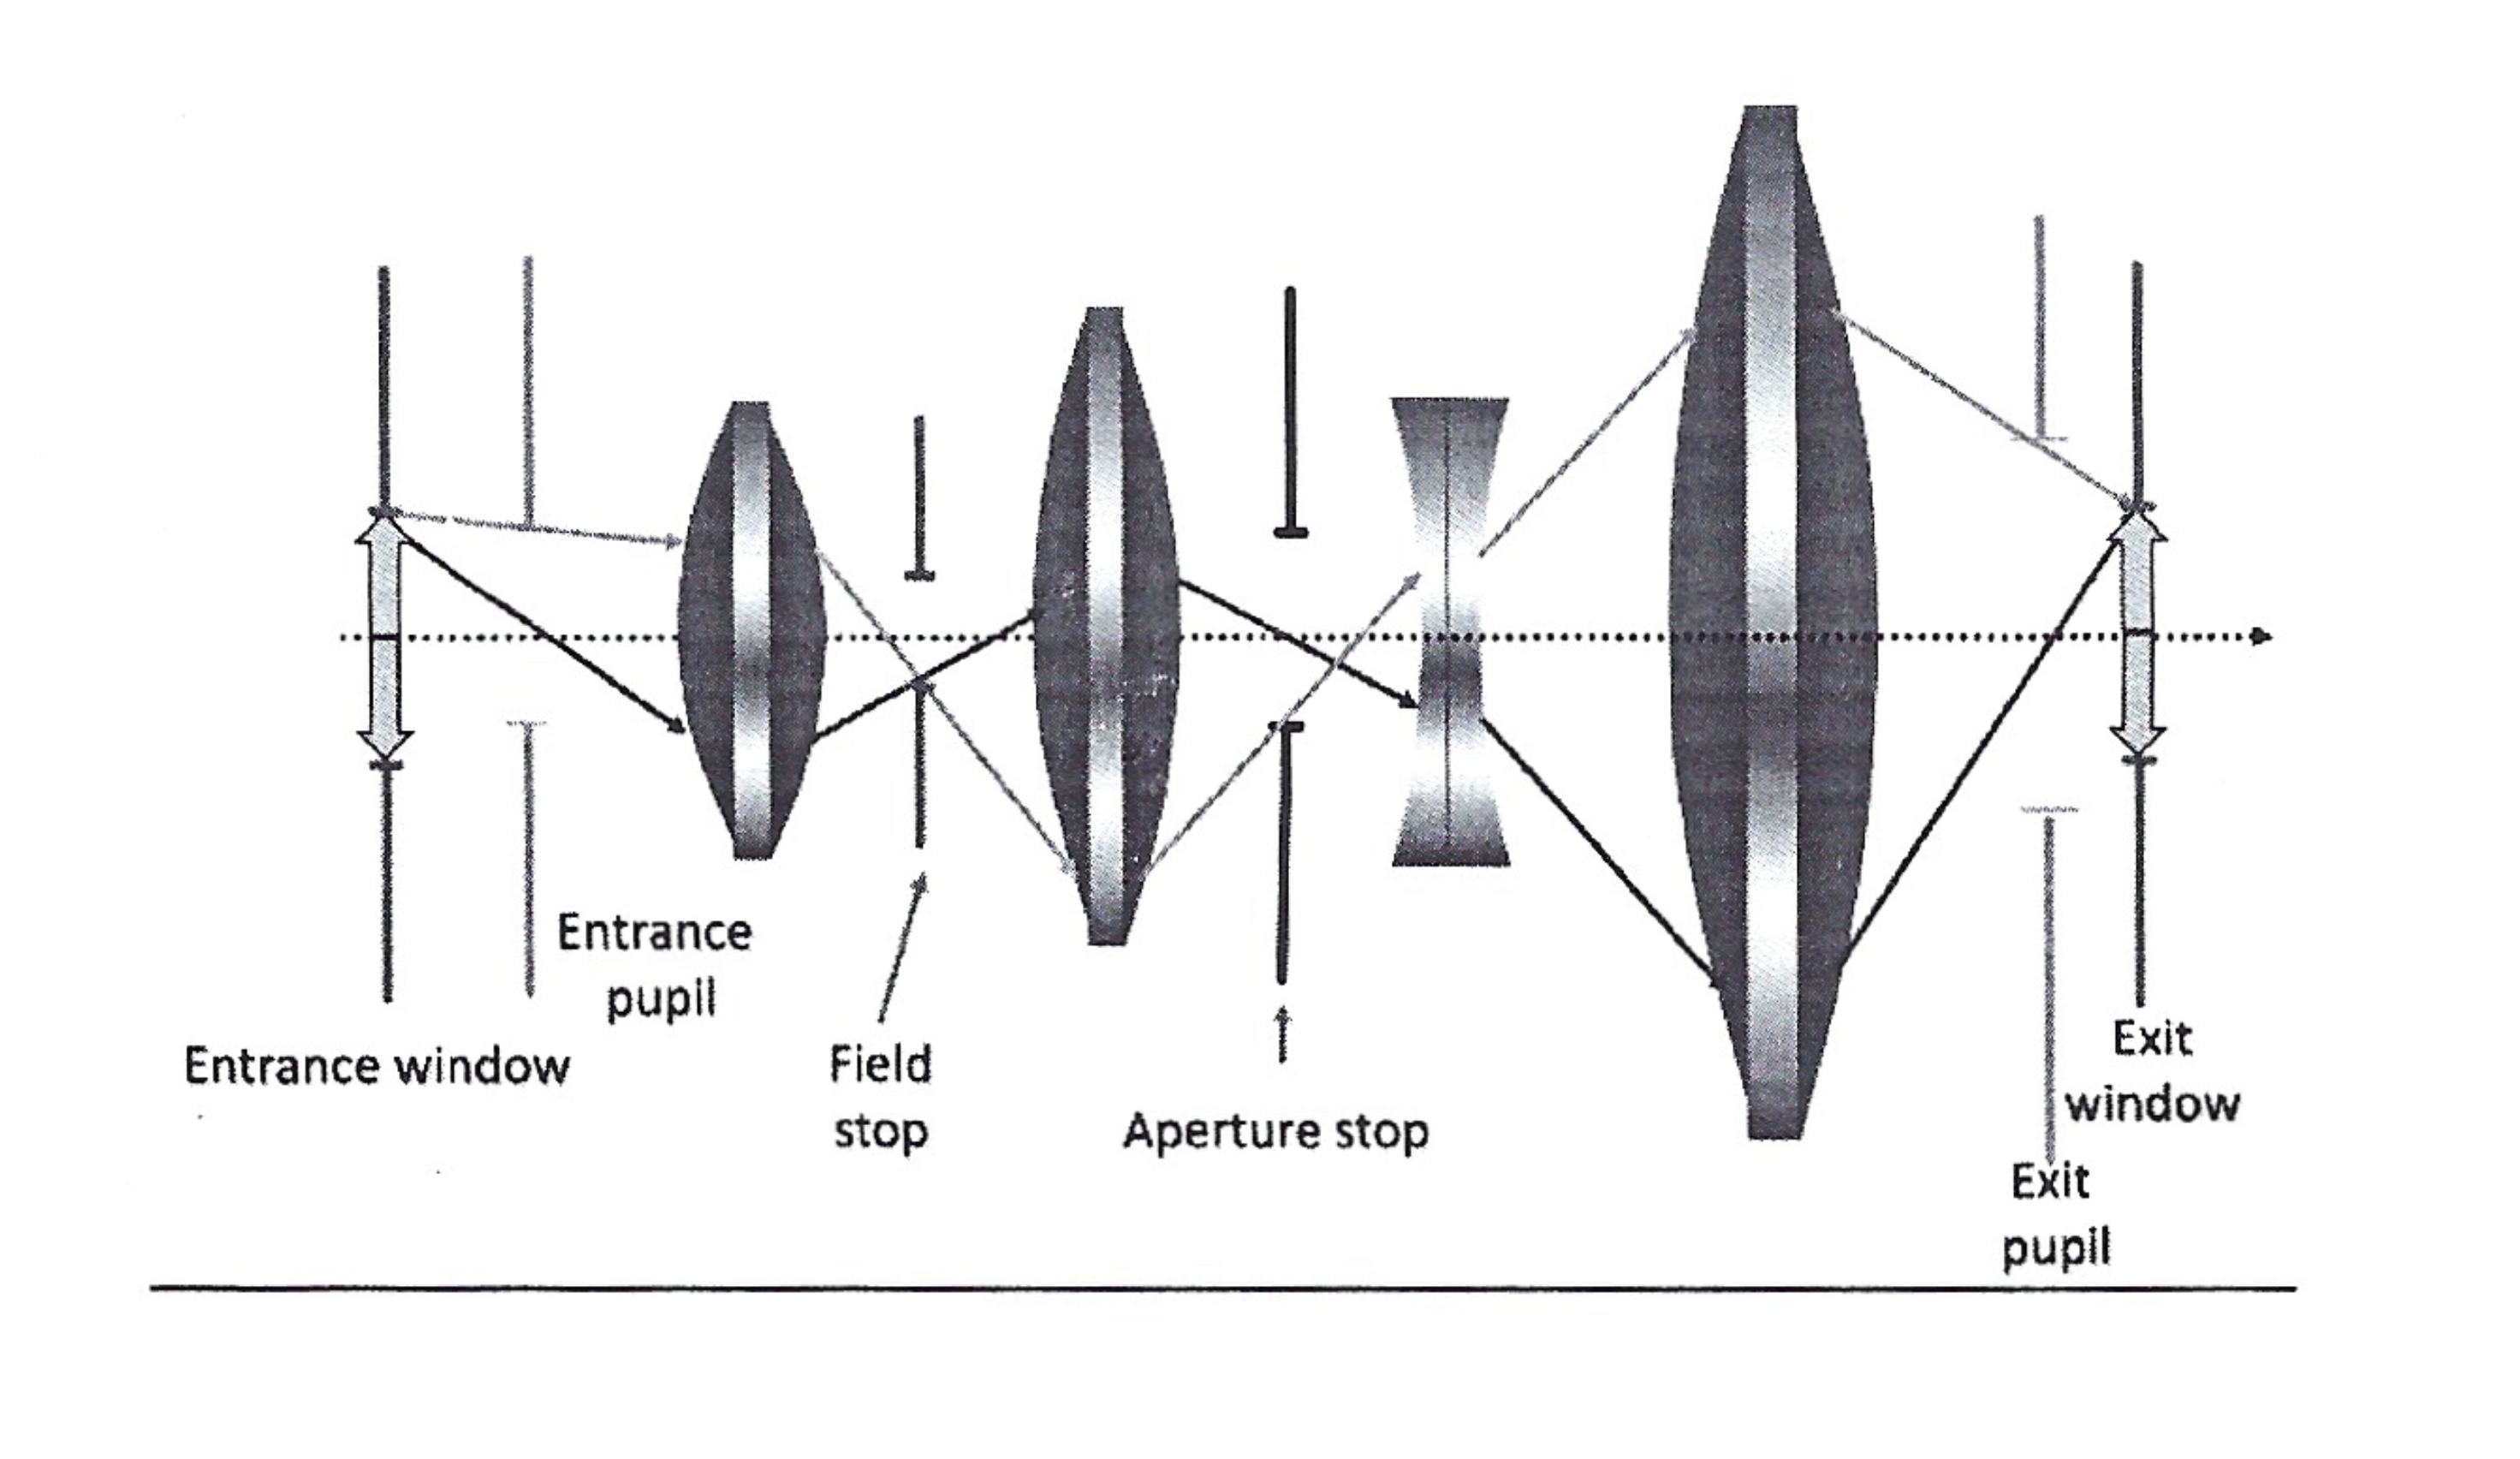
\includegraphics[width=4.0in]{figures/midterm/lens_system.png}}
\caption{Lens System}
\label{fig:m_1}
\end{figure}

% -----------------------------------------------------
% Sixth Problem
% -----------------------------------------------------

\item Find the resultant of \textbf{\underline{superposition}} of the wave E1 and E2 consider that: $E_1 = E_0 \hat{x} \cos (kz - \omega t)$, $E_2 = E_0 \hat{x}\cos(kz = \omega t)$. What does the the result represent? Give a practical example why this case could happen (trasmission line or optics). \textit{(3 points)}\\
 

% -----------------------------------------------------
% Seventh problem
% -----------------------------------------------------

\item Write the phasor of a plane waves of wavelength $\lambda$ and intensity $E_0$ which is propagating along the direction of wave vector $k_1$. Vector $k_1$ lies in the plane $xz$ and forms a 30 degree angle with respect to z. \textit{(4 points)}\\

% -----------------------------------------------------
% Eighth problem
% -----------------------------------------------------

\item An object of height $\SI{10}{C\metre}$ is placed $\SI{50}{c\metre}$ in front of a bi-convex lens with a focal length of $\SI{20}{c\metre}$. Which of the following is true about the image? \textit{(2 points)}\\

\begin{enumerate}[I]
  \item The image is virtual 
  \item The image is situated on the opposite side as the object
  \item The image is inverted
  \begin{enumerate}[A]
    \item I only
    \item I and II only
    \item II and III only
    \item II only
    \item III only
  \end{enumerate}
\end{enumerate}

% -----------------------------------------------------
% Ninth problem
% -----------------------------------------------------

\item Assume that the absolute values of the radii of curvature of the two surfaces of a thin lenses in air are $\SI{10.0}{c\metre}$ and $\SI{5.0}{c\metre}$ and that the index of refraction is 1.5. \textit{(4 points)}\\

\begin{enumerate}[a]
  \item What is the focal length of the lens if both surfaces are convex? 
  \item What is the focal length if one surface is convex and the other concave?
  \item What is the focal length if the lens is double-concave?
  \item Does it matter if we interchange the left and right surface?
\end{enumerate}

% -----------------------------------------------------
% Tenth problem
% -----------------------------------------------------

\item Find the \textbf{\underline{Poynting vector}} S and energy density field for the plane wave field $E = E_0\hat{x}\cos(kz-\omega t)$ traveling in vacuum. (Derive magnetic field first) \textit{(3 points)}\\

\end{enumerate}

\end{comment}

\end{document}